\documentclass[11pt]{exam}
\usepackage[margin=1in]{geometry}
\pagestyle{plain}
\usepackage{amsmath,amsfonts,amssymb,amsthm,enumerate}
\usepackage{multicol}
\usepackage[]{graphicx}
\usepackage{hyperref}
\usepackage{tikz}
\usepackage{pgfplots}
\usepackage{subfigure}
\usepackage[final]{pdfpages}

\everymath{\displaystyle}

\addtolength{\footskip}{2\baselineskip} % to lower the page numbers
\title{\vspace{-0.5in} Math 115 \\ Worksheet Section 6.2}
\date{}


% \theoremstyle{definition}
% \newtheorem{problem}{Problem}
\renewcommand{\questionlabel}{\textbf{Problem~\thequestion.}}
%\printanswers

\begin{document}
\maketitle
\vspace{-0.75in}
If $F'=f$, all antiderivatives of $f$ have the form $F(x)+C$. Thus, we
say \[
  \int f dx = \fillin[F(x) + C]
\]
\begin{questions}
  \question Find an antiderivative of $f(x)=5x-\sqrt{x}$.
    \begin{solution}
      \(\frac{5}{2} x^2 - \frac{2}{3} x^{3/2}\) is an
      antiderivative. Any answer of the form \(\frac{5}{2} x^2 -
      \frac{2}{3} x^{3/2} + C\) is acceptable.
    \end{solution}
  \question Find the general antiderivatives of $g(z)=z+e^z$ and $h(t) = \displaystyle\frac{7}{\cos^2(t)}$.
    \begin{solution}
      \(G(z) = \frac{1}{2} z^2 + e^z + C\) and \(H(t) = 7\tan(t) + C\)
      satisfy \(G'(z) = g(z)\) and \(H'(t) = h(t)\).
    \end{solution}
  \question Find an antiderivative of $p(x)=2+4x+5x^2$ with $F(1)=1$.  Are there any other solutions?
    \begin{solution}
      \(F(x) = 2x + 2x^2 + \frac{5}{3} x^3 - \frac{14}{3} \) is an
      antiderivative of \(p(x)\) with \(F(1) = 1\). There are no other solutions.
    \end{solution}
  \question Find the following indefinite integrals.
    \begin{parts}
    \part $\displaystyle \int \frac{x+1}{x}\ dx$.
    \part \(\int \left( \frac{3}{t} - \frac{2}{t^2} \right) dt\)
    \part \(\int t^3 (t^2+1) dt\)
    \end{parts}
    \begin{solution}
      \begin{enumerate}[(a)]
      \item \(\int \frac{x+1}{x} dx = \int 1 dx + \int \frac{1}{x} dx
        = x + \ln(|x|) + C\)
      \item \(\int \left( \frac{3}{t} - \frac{2}{t^2} \right)dt = 3 \int
        \frac{1}{t} dt - 2 \int \frac{1}{t^2} dt = 3 \ln(|t|) + 2
        t^{-1} + C\)
      \item \(\int t^3(t^2+1) dt = \int t^5 dt + \int t^3 dt =
        \frac{1}{6} t^6 + \frac{1}{4} t^4 + C\)
      \end{enumerate}
    \end{solution}
  \question Find $\displaystyle \int_1^3 \frac{1}{y} \ dy$ and $\displaystyle \int_0^{\pi/4} \sin(t)+\cos(t) \ dt$.
    \begin{solution}
      Since \(\ln(|y|)\) is an antiderivative of \(\frac{1}{y}\), we
      can use the Fundamental Theorem of Calculus to get \[
        \int_1^3 \frac{1}{y} dy = \ln(3)-\ln(1) = \ln(3)
      \]
      Similarly, \(-\cos(t) + \sin(t)\) is an antiderivative of
      \(\sin(t) + \cos(t)\), so we get \[
        \int_0^{\pi/4} \sin(t) + \cos(t) dt = -\cos(\pi/4)+\sin(\pi/4)
        +\cos(0)-\sin(0) = -\frac{\sqrt{2}}{2} + \frac{\sqrt{2}}{2} +1
        - 0 = 1
      \]
    \end{solution}
  \question Water is pumped into a cylindrical tank, standing
    vertically, at a decreasing rate given at time \(t\) minutes by \[
      r(t) = 120 - 6t \text{ cubic feet/min, for } 0 \leq t \leq 10.
    \]
    The tank has radius 5 ft and is empty when \(t=0\). Find the depth
    of water in the tank at \(t=4\).
    \begin{solution}
      The volume of the water in this tank is related to the depth of
      the water by \[
        V = \pi 5^2 d = 25 \pi d \implies d = \frac{V}{25 \pi}
      \]
      Furthermore, the volume of the water over time, \(V(t)\), is
      the antiderivative of \(r(t)\) satisfying \(V(0) = 0\). Thus,
      since \(\int r(t) dt = 120t-3t^2+C\), we get \(V(t) =
      120t-3t^2\) and thus \(h(t) = \frac{1}{25 \pi} V(t) =
      \frac{1}{25 \pi} \left( 120t - 3t^2 \right)\). Thus, \[
        h(4) = \frac{1}{25 \pi} \left( 480 - 48 \right) =
        \frac{438}{25 \pi} \text{ feet} \approx 5.58 \text{ feet}
      \]
    \end{solution}
  \question In drilling an oil well, the total cost, \(C\), consists
    of fixed costs (independent of the depth of the well) and marginal
    costs, which depend on depth; drilling becomes more expensive, per
    meter, deeper into the earth. Suppose the fixed costs are
    \(1,000,000\) riyals and the marginal costs are \[
      C'(x) = 4000 + 10x \text{ riyals/meter}
    \]
    where \(x\) is the depth in meters. Find the total cost of
    drilling a well \(x\) meters deep.
    \begin{solution}
      First, we compute that \[
        \int C'(x) dx = 4000x + 5 x^2 + C
      \]
      Since \(C(0) = 1,000,000\), we have \[
        C(x) = 5x^2 + 4000x + 1000000
      \]
      as the total cost in riyals.
    \end{solution}
  \question The area under the graph of $1/\sqrt{x}$ from $1\leq x \leq b$ is 6.  Find $b$.
    \begin{solution}
      We need to solve \(\int_1^b x^{-1/2} dx = 6\). Since \(2
      x^{1/2}\) is an antiderivative of \(x^{-1/2}\), we get \[
        6 = \int_1^b x^{-1/2} dx = 2 b^{1/2} - 2(1)^{1/2} \implies
        b^{1/2} = 4 \implies b = 16
      \]
    \end{solution}
  \question Sketch the parabola \(y=x(x-\pi)\) and the curve \(y=\sin
    x\), showing their points of intersection. Find the exact area
    between the two graphs.
    \begin{solution}
      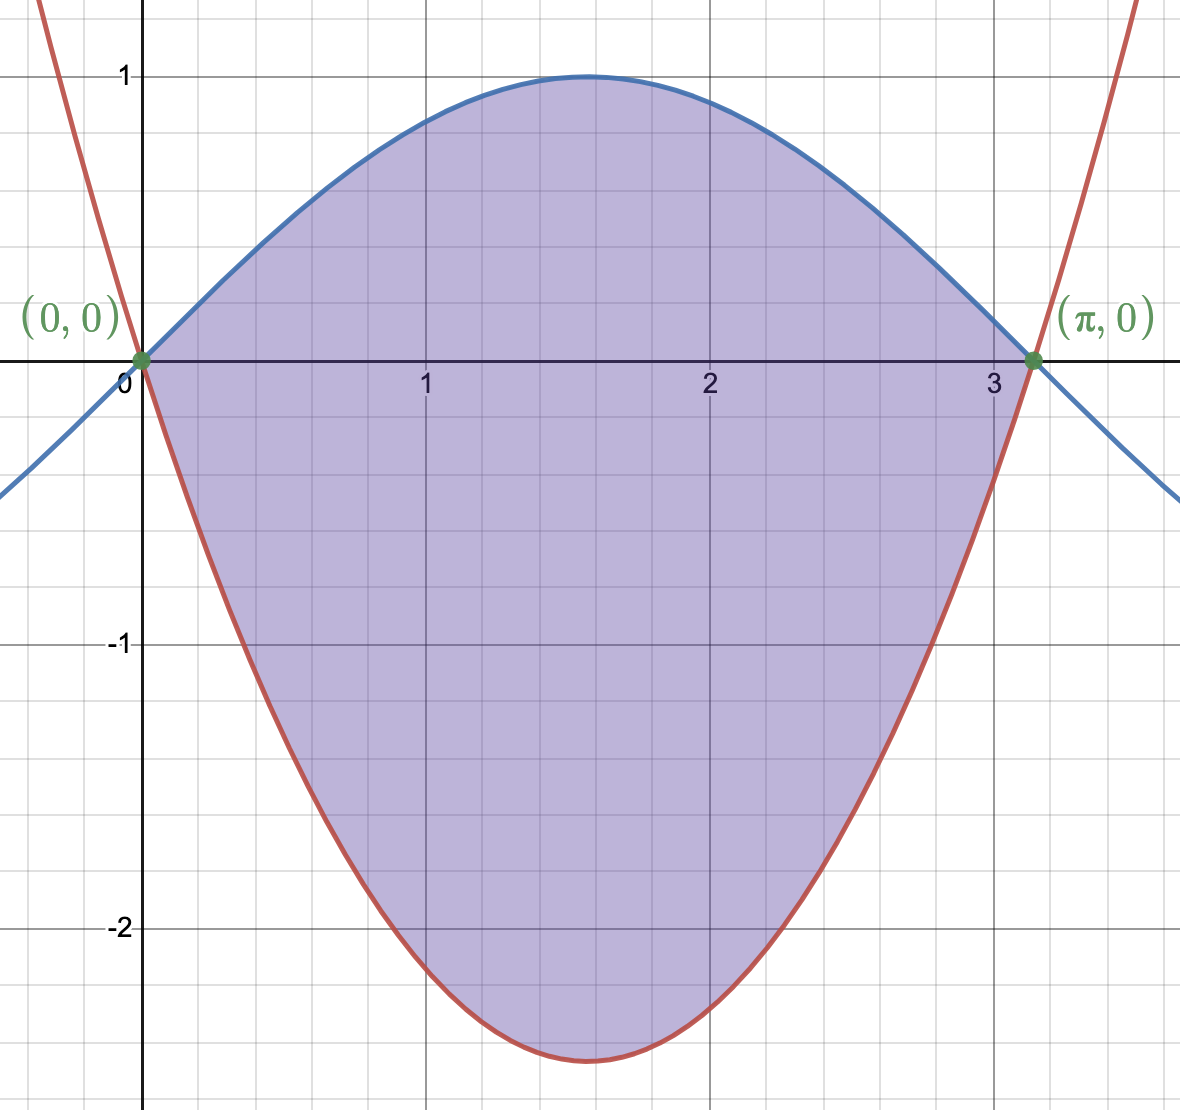
\includegraphics[scale=0.5]{9}

      To compute the area, we must compute the definite integral \[
        \int_0^\pi (\sin x - x(x-\pi)) dx = \int_0^\pi (\sin x - x^2 +
        x\pi) dx
      \]
      This integrand has an antiderivative \(-\cos x - \frac{1}{3} x^3 +
      \frac{\pi}{2} x^2\), so we can compute \[
        \int_0^\pi (\sin x - x(x-\pi)) dx = -\cos(\pi) -
        \frac{\pi^3}{3} + \frac{\pi^3}{2} + \cos(0) + 0 - 0 = 1 +
        \frac{\pi^3}{6} + 1 = 2 + \frac{\pi^3}{6}
      \]
    \end{solution}
   \pagebreak
  \question (Fall 2015 Final Exam)
    Which of the following functions are antiderivatives of \(f(x) =
    \frac{1}{x}\)? Circle all such functions.
    \begin{multicols}{3}
      \begin{enumerate}[(a)]
      \item \(\ln(|x+1|)\)
      \item \(\ln(|x|)\)
      \item \(\ln(|x|)+2\)
      \item \(\ln(4|x|)\)
      \item \(4 \ln(|x|)\)
      \item None of these
      \end{enumerate}
    \end{multicols}
    \begin{solution}
      See \href{https://dhsp.math.lsa.umich.edu/exams/115exam3/f15/s11.pdf}{https://dhsp.math.lsa.umich.edu/exams/115exam3/f15/s11.pdf}
    \end{solution}
  \question Which of the following functions are antiderivatives of
    \(f(x) = e^{x/2}\)?
    \begin{multicols}{3}
      \begin{enumerate}[(a)]
      \item \(e^{x/2}\)
      \item \(2e^{x/2}\)
      \item \(2 e^{(1+x)/2}\)
      \item \(2 e^{x/2} + 1\)
      \item \(e^{x^2/4}\)
      \item None of these
      \end{enumerate}
    \end{multicols}
    \begin{solution}
      (b) and (d) are both antiderivatives of \(f(x)\).
    \end{solution}
  \question (Fall 2013 Final Exam)
A basketball player is running sprints in Crisler Center. She begins in the middle
of the “M” at the center of the court and runs north and south. Her velocity, in meters per
second, for the first 9 seconds is \(v(t) = t \sin (\frac{\pi}
{3} t)\), where \(t\) is the number of seconds since she
started running. She is running north when \(v(t)\) is positive and south when \(v(t)\) is negative.
\begin{parts}
\part Show that the function \[
    f(t) = \frac{9}{\pi^2} \sin \left( \frac{\pi}{3} t \right) -
    \frac{3}{\pi} t \cos\left( \frac{\pi}{3}t \right)
  \]
  is an antiderivative of \(v(t)\).
\part  Where on the court is the player after the 9 seconds? Show all your work and
  give your answer in exact form (no decimal approximations).
\part What is the total distance traveled by the player in the 9 seconds? Show all
your work and give your answer in exact form (no decimal approximations).
\end{parts}
\begin{solution}
  See \href{https://dhsp.math.lsa.umich.edu/exams/115exam3/f13/s8.pdf}{https://dhsp.math.lsa.umich.edu/exams/115exam3/f13/s8.pdf}
\end{solution}
  \question
    \begin{parts}
    \part What is the average value of \(f(t) = \sin t\) over \(0 \leq
      t \leq 2 \pi\)? Why is this a reasonable answer?
    \part Find the average value of \(f(t) = \sin t\) over \(0 \leq t
      \leq \pi\).
    \end{parts}
    \begin{solution}
      \begin{enumerate}[(a)]
      \item We compute \[
          \frac{1}{2\pi} \int_0^{2\pi} \sin (t) dt = \frac{1}{2\pi}
          (-\cos(2\pi)+\cos(0)) = \frac{1}{2\pi}(-1+1) = 0
        \]
        This is reasonable because \(\sin(t)\) oscillates around \(0\)
        with period \(2\pi\).
      \item We compute \[
          \frac{1}{\pi} \int_0^\pi \sin(t) dt =
          \frac{1}{\pi}(-\cos(\pi) + \cos(0)) = \frac{1}{\pi}(1+1) =
         \frac{2}{\pi} 
        \]
      \end{enumerate}
    \end{solution}
  \question Decide if each of the following equalities is true or false.
    \begin{parts}
    \part \(\int e^{2x} dx = 2e^{2x} + C\)
    \part \(\int e^{x^2} dx = 2x \cdot e^{x^2} + C\)
    \part \(\int 3 \cos x dx = 3 \sin x + C\)
    \part \(\int 5 \sin \left( \frac{x}{5} \right) dx = 5 \cos \left(
        \frac{x}{5} \right) + C\)
    \end{parts}
    \begin{solution}
      \begin{enumerate}[(a)]
      \item False. \(\int e^{2x} dx = \frac{1}{2} e^{2x} + C\)
      \item False. \(\frac{d}{dx} \left( 2x e^{x^2} + C \right) = 2
        e^{x^2} + 2x e^{x^2} (2x) = (2+4x^2) e^{x^2}\).
      \item True. \(\frac{d}{dx}(3 \sin x + C) = 3 \cos x\)
      \item False. \(\frac{d}{dx} \left( 5 \cos\left( \frac{x}{5}
          \right) \right) = -\sin\left( \frac{x}{5} \right)\)
      \end{enumerate}
    \end{solution}
\end{questions}
\end{document}
%%% Local Variables:
%%% mode: latex
%%% TeX-master: t
%%% End:
